\documentclass[conference]{IEEEtran}
\usepackage{amsmath,amssymb}
\usepackage{graphicx}
\usepackage{booktabs}
\usepackage{cite}
\usepackage[hidelinks]{hyperref}

\newcommand{\vect}[1]{\mathbf{#1}}
\newcommand{\T}{^{\top}}
\newcommand{\hx}{\hat{\vect{x}}}
\newcommand{\wrap}{\operatorname{wrap}}
\setcounter{dbltopnumber}{3}
\renewcommand{\dbltopfraction}{0.95}
\renewcommand{\textfraction}{0.05}

\begin{document}

\title{Honest Uncertainty in Planar SLAM: Standard and First-Estimates-Jacobian EKF Compared with Graph Optimisation on UTIAS MR.CLAM}

\author{\IEEEauthorblockN{Elya Renom}
\IEEEauthorblockA{McGill University\\ elya.renom@mail.mcgill.ca}}

\maketitle

\begin{abstract}
We build two estimators for planar range-bearing SLAM and run both on the 45 single-robot logs of the UTIAS MR.CLAM dataset, which has motion-capture ground truth. The first is an EKF in a standard form and a First-Estimates-Jacobian (FEJ) form on one code path. The second is a sparse Levenberg--Marquardt graph optimiser, checked against GTSAM. In a 50-run simulation on the MR.CLAM landmark layout the average NEES of the robot pose is 14.9 for the standard EKF, 4.2 for FEJ and 3.2 for an ideal filter, with a 95\% band of $[2.36, 3.72]$. On 40 held-out real runs, with all noise models fitted on dataset~1, the median time-averaged NEES is 19.7, 7.9 and 6.9 for the standard EKF, FEJ and the graph, and the median position RMSE is 0.37, 0.29 and 0.19\,m. The optimiser agrees with GTSAM~4.3 to $10^{-7}$\,m in the poses on 43 of 45 runs. Temporally correlated sensor errors are the largest cause of overconfidence on the real data.
\end{abstract}

\section{Introduction}
An estimator is consistent when the covariance it reports matches the errors it makes. EKF-SLAM is known to become overconfident \cite{bailey2006}, and Huang \emph{et al.} traced a primary cause to observability: the linearised system used by the filter has one unobservable direction fewer than the true system, so the filter gains information that the measurements do not carry \cite{huang2008,huang2010}. Their First-Estimates-Jacobian (FEJ) filter restores the correct unobservable subspace.

This paper reproduces that failure and its correction, then asks how much of it carries over to real data. The contributions are: (i) an EKF-SLAM with standard, FEJ and ideal Jacobians on one code path, with a unit test that checks the unobservable subspace directly; (ii) a sparse graph optimiser whose cost, estimates and marginal covariances are compared with GTSAM under two pose-error conventions; (iii) a calibration and evaluation protocol on MR.CLAM \cite{leung2011} in which every parameter is fitted on dataset~1 and frozen before datasets 2--9 are processed; (iv) results on all 45 runs, including the runs where the methods fail.

\section{Models}
The state holds the robot pose and $N$ landmark positions, $\vect{x} = [x_r, y_r, \theta, m_{1x}, m_{1y}, \dots]\T \in \mathbb{R}^{3+2N}$. Odometry is a forward and angular velocity $\vect{u} = (v, \omega)$, applied once per sample of length $\Delta t$:
\begin{equation}
\begin{aligned}
x_r &\leftarrow x_r + v\Delta t\cos\theta, \qquad y_r \leftarrow y_r + v\Delta t\sin\theta,\\
\theta &\leftarrow \wrap(\theta + \omega\Delta t).
\end{aligned}
\end{equation}
With $\vect{J} = \bigl[\begin{smallmatrix}0 & -1\\ 1 & 0\end{smallmatrix}\bigr]$ and robot position $\vect{p}$, the Jacobians with respect to the pose and the control are
\begin{equation}
\vect{G} = \begin{bmatrix} \vect{I}_2 & \vect{J}(\vect{p}_{k+1} {-} \vect{p}_k)\\ \vect{0} & 1 \end{bmatrix}\!,\;
\vect{V} = \Delta t\!\begin{bmatrix} \cos\theta & 0\\ \sin\theta & 0\\ 0 & 1 \end{bmatrix}\!,
\label{eq:G}
\end{equation}
where $\vect{J}(\vect{p}_{k+1}-\vect{p}_k) = [-v\Delta t\sin\theta,\; v\Delta t\cos\theta]\T$. Control noise is $\vect{M} = \operatorname{diag}(\sigma_v^2, \sigma_\omega^2)$. A sighting of landmark $j$ gives range and bearing. With $\boldsymbol{\delta} = \vect{m}_j - \vect{p}$ and $q = \boldsymbol{\delta}\T\boldsymbol{\delta}$,
\begin{equation}
h(\vect{x}) = \begin{bmatrix} \sqrt{q}\\ \wrap(\operatorname{atan2}(\delta_y, \delta_x) - \theta)\end{bmatrix},
\end{equation}
\begin{equation}
\vect{H}_m = \begin{bmatrix} \delta_x/\sqrt{q} & \delta_y/\sqrt{q}\\ -\delta_y/q & \delta_x/q \end{bmatrix},\quad
\vect{H}_r = \vect{H}_m\begin{bmatrix} -\vect{I}_2 & -\vect{J}\boldsymbol{\delta}\end{bmatrix},
\label{eq:Hr}
\end{equation}
with noise $\vect{R} = \operatorname{diag}(\sigma_r^2, \sigma_\phi^2)$. The full Jacobian $\vect{H}$ has five non-zero columns. Every analytic Jacobian in the code is tested against central differences with step $10^{-6}$.

\section{EKF-SLAM and the FEJ Variant}
\subsection{Filter}
\emph{Predict.} Only the robot block and the robot-to-map cross terms change, so a step costs $O(N)$:
$\vect{P}_{rr} \leftarrow \vect{G}\vect{P}_{rr}\vect{G}\T + \vect{V}\vect{M}\vect{V}\T$, $\vect{P}_{rm} \leftarrow \vect{G}\vect{P}_{rm}$.
The MR.CLAM odometry stamps are irregular and steps are split at measurement times, so the code uses $\vect{Q}_k = \Delta t_k\,\Delta t_{\mathrm{nom}}\,\hat{\vect{V}}\vect{M}\hat{\vect{V}}\T$ with $\hat{\vect{V}} = \vect{V}/\Delta t$. This equals $\vect{V}\vect{M}\vect{V}\T$ at the nominal 15\,ms and is additive when a step is split.

\emph{New landmark.} The first sighting $(r, \phi)$ is inverted, $\vect{m} = \vect{p} + r[\cos(\theta+\phi), \sin(\theta+\phi)]\T$, and the covariance is extended with $\vect{J}_x = [\vect{I}_2,\; \vect{J}(\vect{m}-\vect{p})]$ and $\vect{J}_z = \partial\vect{m}/\partial(r,\phi)$: $\vect{P}_{\mathrm{new,new}} = \vect{J}_x\vect{P}_{rr}\vect{J}_x\T + \vect{J}_z\vect{R}\vect{J}_z\T$ and $\vect{P}_{\mathrm{new,rest}} = \vect{J}_x\vect{P}_{r,\mathrm{rest}}$.

\emph{Update.} With innovation $\boldsymbol{\nu} = \vect{z} - h(\hx)$ (bearing wrapped) and $\vect{S} = \vect{H}\vect{P}\vect{H}\T + \vect{R}$, a measurement is skipped when $\boldsymbol{\nu}\T\vect{S}^{-1}\boldsymbol{\nu} > 9.21$, the 99\% point of $\chi^2_2$. Otherwise $\vect{K} = \vect{P}\vect{H}\T\vect{S}^{-1}$ is obtained from a Cholesky solve and $\vect{P} \leftarrow (\vect{I}-\vect{K}\vect{H})\vect{P}(\vect{I}-\vect{K}\vect{H})\T + \vect{K}\vect{R}\vect{K}\T$, followed by symmetrisation. Measurements that share a timestamp form one batch: new landmarks are initialised first, from the predicted pose, then known landmarks are updated one at a time.

\subsection{Why the standard filter gains spurious information}
The error state obeys $\tilde{\vect{x}}_{k+1} \approx \boldsymbol{\Phi}_k\tilde{\vect{x}}_k$ with $\boldsymbol{\Phi}_k = \operatorname{blkdiag}(\vect{G}_k, \vect{I})$, and $\tilde{\vect{z}}_k \approx \vect{H}_k\tilde{\vect{x}}_k$. Consider
\begin{equation}
\vect{N}_k = \begin{bmatrix} \vect{I}_2 & \vect{J}\vect{p}_k\\ \vect{0} & 1\\ \vect{I}_2 & \vect{J}\vect{m}_1\\ \vdots & \vdots \end{bmatrix}.
\label{eq:N}
\end{equation}
Its columns are a shift of the whole map in $x$, a shift in $y$, and a rotation about the origin: the three degrees of freedom of the global frame, which range and bearing cannot sense. When all Jacobians are evaluated at one consistent set of states, \eqref{eq:G} gives $\boldsymbol{\Phi}_k\vect{N}_k = \vect{N}_{k+1}$, because $\vect{J}\vect{p}_k + \vect{J}(\vect{p}_{k+1}-\vect{p}_k) = \vect{J}\vect{p}_{k+1}$, and \eqref{eq:Hr} gives $\vect{H}_k\vect{N}_k = \vect{H}_m[-\vect{J}\vect{p}_k - \vect{J}(\vect{m}-\vect{p}_k) + \vect{J}\vect{m}] = \vect{0}$. Hence $\vect{H}_k\boldsymbol{\Phi}_{k-1}\cdots\boldsymbol{\Phi}_0\vect{N}_0 = \vect{0}$ for all $k$: the observability matrix has a null space of dimension three and no measurement adds information along it \cite{huang2010}.

The standard EKF evaluates $\vect{G}_k$ with $\hat{\vect{p}}_{k+1|k} - \hat{\vect{p}}_{k|k}$ and $\vect{H}_k$ with $\hat{\vect{p}}_{k|k-1}$ and $\hat{\vect{m}}_{k|k-1}$. The same pose then enters with two values, before and after its update, and each landmark enters with a new value at every step. The sums above no longer cancel in the rotation column, the null space keeps only the two translations, and each update reduces the variance of the global orientation without evidence \cite{huang2008}. Bailey \emph{et al.} observed the same effect empirically and reported that it becomes visible once the heading standard deviation exceeds one to two degrees \cite{bailey2006}.

\subsection{FEJ rule and implementation}
FEJ evaluates every Jacobian at the first estimate of each variable: a landmark at the value it received when it was initialised, $\vect{m}^{\circ}_j$, and pose $k$ at its predicted value $\hat{\vect{p}}_{k|k-1}$. The only changes are
\begin{align}
\vect{G}_k &: \; \vect{J}(\hat{\vect{p}}_{k+1|k} - \hat{\vect{p}}_{k|k-1}) \text{ in place of } \vect{J}(\hat{\vect{p}}_{k+1|k} - \hat{\vect{p}}_{k|k}),\\
\vect{H}_k &: \; \boldsymbol{\delta} = \vect{m}^{\circ}_j - \hat{\vect{p}}_{k|k-1}.
\end{align}
The mean is still propagated from the updated pose and the innovation still uses the latest estimates. In code, each Jacobian takes its linearisation point as an argument, and the filter keeps a copy of the predicted pose that updates never overwrite. Three details matter in practice. First, MR.CLAM has many odometry steps between sightings; a step that follows no update is identical in both filters, so only the first prediction after an update differs, and the product of the $\vect{G}$ matrices still telescopes. Second, all landmarks in one batch share the same robot linearisation point. Third, a new landmark is initialised from the predicted pose, so its row of \eqref{eq:N} is exactly $[\vect{I}_2,\; \vect{J}\vect{m}^{\circ}_j]$.

A unit test replays the Jacobians the filter applied to $\vect{P}$ and propagates $\vect{N}_k$ alongside. In FEJ mode, and in an ideal mode that uses the true state, $\max|\vect{H}_k\vect{N}_k| < 10^{-14}$ over one simulated lap and $\vect{N}_k\T\vect{P}^{-1}\vect{N}_k$ is unchanged by every update. In standard mode the rotation column of $\vect{H}_k\vect{N}_k$ reaches 0.26, and the updates add $4.8\times10^{3}$\,rad$^{-2}$ of information along the rotation, about one third of what the filter holds at the end of the lap.

\section{Consistency Measures}
With pose error $\vect{e}_k$ (heading wrapped) and innovation $\boldsymbol{\nu}_k$,
\begin{equation}
\mathrm{NEES}_k = \vect{e}_k\T\vect{P}_k^{-1}\vect{e}_k,\qquad \mathrm{NIS}_k = \boldsymbol{\nu}_k\T\vect{S}_k^{-1}\boldsymbol{\nu}_k .
\end{equation}
For a consistent filter NEES follows $\chi^2_3$ and NIS follows $\chi^2_2$, with means 3 and 2 \cite{barshalom2001}. A single sample lies in $[0.22, 9.35]$ (NEES) or $[0.05, 7.38]$ (NIS) with probability 0.95. Over $n$ independent runs, $n$ times the average NEES at a fixed time is $\chi^2_{3n}$, which gives the band $[2.36, 3.72]$ for $n = 50$. A 99\% gate truncates the NIS of accepted measurements, whose expectation becomes 1.91.

Real runs cannot be repeated, and NEES samples within one run are correlated. For each run we therefore report the time-averaged NEES and the fraction of samples inside $[0.22, 9.35]$, and we summarise both over runs. The Vicon covariance is added to $\vect{P}$ before the NEES is formed.

\section{Graph-SLAM}
\subsection{Factors}
The variables are one pose $\vect{X}_k$ per measurement timestamp and the landmarks $\vect{L}_j$. A prior fixes $\vect{X}_0$ at the ground-truth start pose with standard deviation 1\,mm and $10^{-3}$\,rad, which removes the three unobservable degrees of freedom. The filter starts from the same pose and covariance.

\emph{Odometry factors.} The samples between two keyframes are integrated in the frame of $\vect{X}_k$, starting from the zero pose with zero covariance and applying the EKF's own prediction, $\boldsymbol{\Sigma} \leftarrow \vect{G}\boldsymbol{\Sigma}\vect{G}\T + \vect{Q}$. Two points need care. $\vect{V}\vect{M}\vect{V}\T$ has rank two, so a short or stationary interval gives a singular $\boldsymbol{\Sigma}$; a small noise rate, $(1\,\mathrm{mm})^2$ and $(0.1^\circ)^2$ per second, is added in the filter and in the pre-integration alike. Also, the recursion expresses $\boldsymbol{\Sigma}$ in the frame of $\vect{X}_k$, while the residual below is expressed in the end frame, so the factor uses $\boldsymbol{\Sigma}_e = \vect{T}\boldsymbol{\Sigma}\vect{T}\T$ with $\vect{T} = \operatorname{blkdiag}(\vect{R}_z\T, 1)$. A Monte Carlo test confirms that the whitened residual at the true poses has mean 3.0 with $\boldsymbol{\Sigma}_e$ and exceeds 4 with $\boldsymbol{\Sigma}$ for a turning interval.

With measurement $\vect{z} = (\vect{t}_z, \theta_z)$ the pose-pose residual of \cite{grisetti2010} is
\begin{equation}
\vect{e}_{ij} = \begin{bmatrix} \vect{R}_z\T\bigl(\vect{R}_i\T(\vect{t}_j - \vect{t}_i) - \vect{t}_z\bigr)\\ \wrap(\theta_j - \theta_i - \theta_z)\end{bmatrix},
\label{eq:between}
\end{equation}
\begin{equation}
\begin{aligned}
\vect{A}_{ij} &= \begin{bmatrix} -\vect{R}_z\T\vect{R}_i\T & \vect{R}_z\T\tfrac{\partial\vect{R}_i\T}{\partial\theta_i}(\vect{t}_j - \vect{t}_i)\\ \vect{0} & -1\end{bmatrix},\\
\vect{B}_{ij} &= \begin{bmatrix} \vect{R}_z\T\vect{R}_i\T & \vect{0}\\ \vect{0} & 1\end{bmatrix}.
\end{aligned}
\end{equation}

\emph{Bearing-range factors.} The residual is $\vect{e} = h(\vect{X}_k, \vect{L}_j) - \vect{z}$, so its Jacobians are $\vect{H}_r$ and $\vect{H}_m$ and the EKF code is reused.

\subsection{Optimiser}
The cost is $F = \sum \vect{e}\T\boldsymbol{\Omega}\vect{e}$ with $\boldsymbol{\Omega} = \boldsymbol{\Sigma}^{-1}$. Each iteration forms $\vect{H} = \sum\vect{J}\T\boldsymbol{\Omega}\vect{J}$ and $\vect{b} = \sum\vect{J}\T\boldsymbol{\Omega}\vect{e}$ from triplets, with all factors of one type linearised in a single vectorised call, and solves $(\vect{H} + \lambda\operatorname{diag}\vect{H})\Delta\vect{x} = -\vect{b}$ with a sparse direct solver \cite{dellaert2017}. $\lambda$ is divided by 10 after a step that lowers $F$ and multiplied by 10 otherwise; the iteration stops when the largest component of an accepted step is below $10^{-6}$. Gauss--Newton is the same loop with $\lambda = 0$.

The covariance of a variable is its block of $\vect{H}^{-1}$ at the solution. For an odometry chain these blocks are available exactly in $O(K)$: with $\vect{H} = \bigl[\begin{smallmatrix}\vect{A} & \vect{B}\\ \vect{B}\T & \vect{C}\end{smallmatrix}\bigr]$ ordered poses then landmarks, $\vect{A}$ is block-tridiagonal and $\vect{C}$ is at most $30\times30$, so $\boldsymbol{\Sigma}_{ll} = (\vect{C} - \vect{B}\T\vect{A}^{-1}\vect{B})^{-1}$ and $\boldsymbol{\Sigma}_{pp} = \vect{A}^{-1} + \vect{A}^{-1}\vect{B}\boldsymbol{\Sigma}_{ll}\vect{B}\T\vect{A}^{-1}$, where the diagonal blocks of $\vect{A}^{-1}$ follow from a two-sweep recursion. The result is tested against a dense inverse. With $M$ bearing-range factors and $L$ landmarks the residual dimension exceeds the variable dimension by $2M - 2L$, and $F/(2M-2L)$ is near 1 for correct noise; over 40 simulated graphs its mean is within 0.06 of 1.

Measurements are selected without ground truth. The graph starts from the measurements the FEJ filter accepted and from its trajectory; after each solve every measurement of a mapped landmark is tested at the solution with threshold 9.21, and the factor set is rebuilt until it stops changing.

\subsection{The same graph in GTSAM}
The graph is rebuilt with \texttt{PriorFactorPose2}, \texttt{BetweenFactorPose2} with covariance $\boldsymbol{\Sigma}_e$, and \texttt{BearingRangeFactor2D}, whose measurement and noise list the bearing first. Three conventions matter. GTSAM reports $\tfrac12 F$. \texttt{Marginals} returns a pose covariance in the body frame, which we rotate with $\operatorname{blkdiag}(\vect{R}(\theta), 1)$ before comparing it with the blocks of $\vect{H}^{-1}$. Finally, the pose error depends on the version. GTSAM~4.2 uses the components of $\vect{z}^{-1}(\vect{X}_i^{-1}\vect{X}_j)$, which is exactly \eqref{eq:between}, and linearises it without the Jacobian of its chart. GTSAM~4.3 uses the SE(2) logarithm of that pose with exact Jacobians. Our optimiser therefore offers a second residual, $\vect{e}' = \operatorname{Log}(\vect{e}_{ij})$, whose Jacobians are $\vect{D}\vect{A}_{ij}$ and $\vect{D}\vect{B}_{ij}$ with $\vect{D} = \partial\operatorname{Log}/\partial\vect{e}$. The two residuals agree to first order and differ by terms of order $|\theta_e|\,\|\vect{t}_e\|$.

\section{Experiments}
\subsection{Simulation}
The simulator uses the 15 MR.CLAM landmark positions. The robot drives 10 laps of a rounded rectangle at 0.2\,m/s (139\,s per lap) with odometry at 67\,Hz and measurements at about 5\,Hz. Controls carry noise $\sigma_v = 0.05$\,m/s and $\sigma_\omega = 0.1$\,rad/s per sample, measurements $\sigma_r = 0.1$\,m. Ranges are limited to 0.8--3\,m; the lower limit is the shortest range in the real data, and without it passes within 0.25\,m of a landmark made the FEJ filter diverge. A start pose known to 1\,mm in a small room keeps the heading uncertainty low, so the configuration was chosen by a criterion fixed beforehand: sweep sensing range $\{3, 2\}$\,m, $\sigma_\omega \in \{0.1, 0.2\}$\,rad/s and $\sigma_\phi \in \{2, 5, 10\}^\circ$ in that order and take the first point where the ideal filter's heading standard deviation reaches $3^\circ$ before the first loop closure. This selected 3\,m, 0.1\,rad/s and $10^\circ$ ($3.5^\circ$ of heading uncertainty). Huang \emph{et al.} also used noise above typical practice, with a $10^\circ$ bearing sigma in their range-bearing study \cite{huang2010}.

Fig.~\ref{fig:anees} shows the result of 50 runs with the gate off, so the three filters process identical measurements. The ideal filter averages 3.2 and lies inside the band 90\% of the time. The standard EKF leaves the band within the first lap, averages 14.9 and is above the band 99\% of the time; its dips coincide with the return to the start area. FEJ averages 4.2 and lies inside the band 31\% of the time. Position RMSE is 0.18, 0.39 and 0.20\,m for ideal, standard and FEJ. With the gate on the averages are 3.3, 16.4 and 3.5. Across the 12 swept configurations the standard filter's ANEES ranges from 3.4 to 64 and grows with the heading uncertainty. With 3\,m range FEJ stays between 3.0 and 3.3. With 2\,m range and $\sigma_\omega = 0.2$\,rad/s the ideal filter itself leaves the band (4.3--4.7) and FEJ diverged at two of the three points: first estimates taken under strong nonlinearity are poor linearisation points, a known cost of the method \cite{huang2010}.

\begin{figure}[t]
\centering
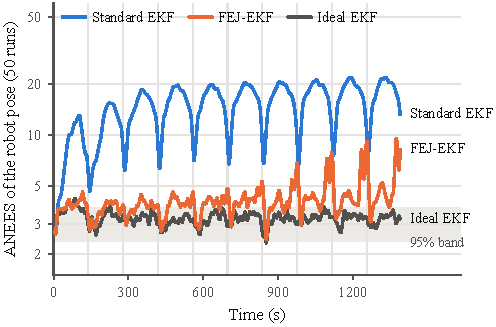
\includegraphics[width=\columnwidth]{figures/fig_anees.pdf}
\caption{Average NEES of the robot pose over 50 simulated runs (10\,s moving average). The shaded region is the 95\% band $[2.36, 3.72]$; vertical lines mark laps.}
\label{fig:anees}
\end{figure}

\subsection{Real data: calibration on dataset 1}
Each MR.CLAM robot log is treated as one SLAM problem: barcodes are mapped to subjects per dataset, sightings of other robots are dropped, and the run starts at the ground-truth pose. All parameters below were fitted on dataset~1, written to one file and committed before any estimator was run on datasets 2--9; its hash is stored with every result.

\emph{Odometry.} The logged odometry is the commanded velocity. Comparing 1\,s windows with ground truth gave, consistently for the five robots, a delay of 0.14--0.24\,s, a turn-rate gain of 0.91--0.96, and a forward speed that drops while turning, $v' = s_v v - c_v|\omega|$ with $s_v \approx 1.05$ and $c_v \approx 0.09$\,m. The remaining heading error is four to five times larger within 0.5\,s of a commanded turn, so $\vect{M}$ takes two values: $\sigma_\omega$ of 0.05--0.14 (straight) and 0.30--0.44\,rad/s (turning) per 15\,ms sample. These come from the standard deviation of the window error. A filter using a robust (MAD) sigma diverged on dataset~1, because control errors cannot be gated.

\begin{figure}[t]
\centering
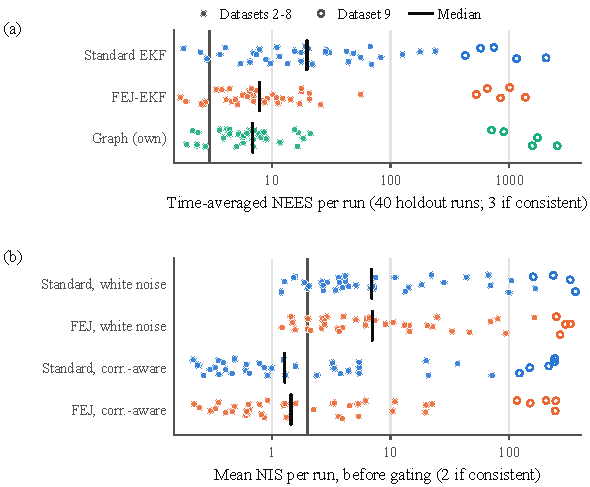
\includegraphics[width=\columnwidth]{figures/fig_consistency.pdf}
\caption{Spread over the 40 held-out runs. (a) Time-averaged NEES per run. (b) Mean NIS per run for the two measurement-noise models.}
\label{fig:consistency}
\end{figure}

\emph{Camera.} Measurement residuals against ground truth give, per robot, a bearing sigma of 0.006--0.017\,rad from the median absolute deviation and a range sigma that grows with distance, $\sigma_r = c_0 + c_1 r$ with $c_1$ between 0.016 and 0.051 and bootstrap intervals that exclude zero. A 40\,ms latency and a small lever arm are corrected. The residuals are strongly correlated in time: the mean of the residuals to one landmark over a 10\,s block is 2.3--4.2 times (range) and 1.9--2.9 times (bearing) more spread than white noise allows. The sigmas are inflated by these factors, which are computed from the residuals alone with no filter in the loop, and sightings taken while the robot is commanded to stand still are dropped.

\emph{Data issues.} In dataset~1 the ground-truth positions of two landmarks are exchanged; the loader detects and corrects this, which affects scoring only. Dataset~8 maps 14 landmarks. Ground truth has gaps of up to 662\,s, which are excluded from scoring.

\subsection{Real data: results}
Table~\ref{tab:accuracy} gives accuracy and NEES, and Fig.~\ref{fig:consistency} the spread over runs. On the 40 held-out runs the median time-averaged NEES is 19.7 for the standard EKF, 7.9 for FEJ and 6.9 for the graph, and the median fraction of NEES samples inside $[0.22, 9.35]$ is 30\%, 77\% and 82\%. FEJ has the lower NEES in 35 of 40 runs and the lower position RMSE in 32. At the final pose, where filter and smoother condition on the same data, the median NEES is 28.5, 7.1 and 5.3. No method reaches 3: the remaining overconfidence comes from sensor errors that the models treat as white.

\begin{table*}[t]
\caption{Accuracy and consistency on MR.CLAM: median [interquartile range] over runs. Datasets 2--9 are held out; dataset 1 was used for calibration. NEES is the time average per run (3 if consistent); filter values are filtered, graph values are smoothed. The own graph uses the Grisetti residual and GTSAM~4.3 its log-map residual.}
\label{tab:accuracy}
\centering
\footnotesize
\setlength{\tabcolsep}{5pt}
\begin{tabular}{@{}llccccc@{}}
\toprule
Datasets & Method & Position RMSE (m) & After alignment (m) & Heading RMSE (deg) & Landmark RMSE (m) & NEES \\
\midrule
2--9 (40 runs) & Standard EKF & 0.37 [0.20, 0.79] & 0.11 [0.08, 0.32] & 6.4 [3.2, 18.1] & 0.42 [0.21, 0.97] & 19.7 [7.8, 68.0] \\
 & FEJ-EKF & 0.29 [0.15, 0.45] & 0.12 [0.06, 0.37] & 5.7 [2.6, 12.2] & 0.21 [0.14, 0.48] & 7.9 [4.9, 17.7] \\
 & Graph (own) & 0.19 [0.11, 0.36] & 0.05 [0.04, 0.07] & 3.0 [1.8, 6.2] & 0.19 [0.12, 0.45] & 6.9 [4.4, 12.7] \\
 & Graph (GTSAM) & 0.22 [0.11, 0.36] & 0.05 [0.04, 0.07] & 3.2 [1.7, 6.2] & 0.19 [0.12, 0.45] & 7.0 [4.5, 12.7] \\
\midrule
2--8 (35 runs) & Standard EKF & 0.33 [0.19, 0.65] & 0.10 [0.08, 0.17] & 5.6 [3.0, 13.7] & 0.39 [0.19, 0.63] & 17.6 [7.3, 43.5] \\
 & FEJ-EKF & 0.25 [0.12, 0.39] & 0.09 [0.06, 0.17] & 5.2 [2.2, 8.8] & 0.18 [0.13, 0.34] & 7.0 [4.5, 11.8] \\
 & Graph (own) & 0.16 [0.10, 0.27] & 0.05 [0.04, 0.06] & 2.6 [1.7, 4.6] & 0.16 [0.11, 0.34] & 6.2 [4.4, 8.4] \\
 & Graph (GTSAM) & 0.16 [0.10, 0.27] & 0.05 [0.04, 0.06] & 2.6 [1.5, 5.0] & 0.17 [0.12, 0.34] & 6.5 [4.3, 8.5] \\
\midrule
9 (5 runs) & Standard EKF & 10.30 [8.61, 10.95] & 6.23 [4.28, 7.87] & 106.4 [90.5, 110.3] & 6.29 [3.55, 7.32] & 743.5 [573.2, 1152.7] \\
 & FEJ-EKF & 7.55 [6.67, 8.89] & 5.14 [4.28, 6.33] & 100.4 [89.6, 105.0] & 7.35 [4.60, 7.46] & 844.3 [652.5, 1009.7] \\
 & Graph (own) & 6.71 [5.78, 8.24] & 4.24 [3.73, 5.31] & 99.2 [89.2, 105.5] & 7.15 [4.64, 7.47] & 1565.2 [900.1, 1730.3] \\
 & Graph (GTSAM) & 6.92 [5.77, 8.31] & 4.43 [3.73, 5.19] & 99.2 [89.2, 105.0] & 7.15 [4.64, 7.33] & 1565.1 [899.0, 1712.1] \\
\midrule
1 (5 runs) & Standard EKF & 0.17 [0.14, 0.43] & 0.09 [0.07, 0.13] & 3.6 [2.8, 5.6] & 0.19 [0.18, 0.45] & 5.7 [5.4, 15.1] \\
 & FEJ-EKF & 0.37 [0.14, 0.41] & 0.10 [0.05, 0.13] & 4.8 [3.3, 6.0] & 0.51 [0.12, 0.51] & 8.8 [4.3, 12.6] \\
 & Graph (own) & 0.38 [0.07, 0.41] & 0.04 [0.03, 0.04] & 5.1 [1.6, 6.1] & 0.46 [0.10, 0.51] & 8.4 [5.5, 14.3] \\
 & Graph (GTSAM) & 0.38 [0.07, 0.41] & 0.04 [0.03, 0.04] & 5.2 [1.5, 6.0] & 0.46 [0.10, 0.51] & 8.3 [5.5, 14.2] \\
\bottomrule
\end{tabular}

\end{table*}

\begin{figure*}[t]
\centering
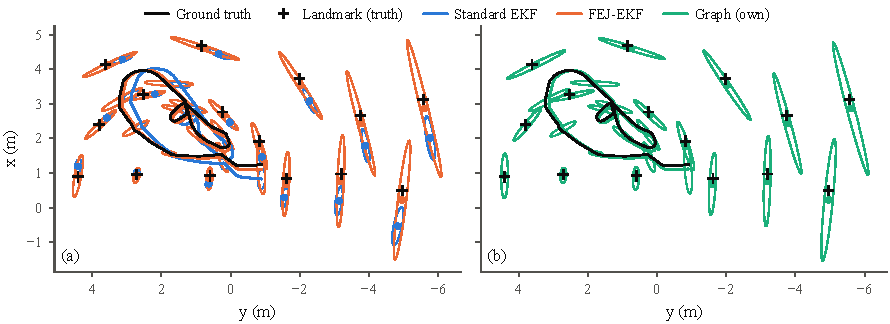
\includegraphics[width=\textwidth]{figures/fig_map.pdf}
\caption{Dataset 4, robot 3, the held-out run with the median standard-EKF error: a four-minute stretch of the trajectory, final landmark estimates and 3$\sigma$ ellipses. (a) Standard and FEJ EKF. (b) Own graph optimiser. The landmark ellipses are elongated around the start pose, which shows the uncertainty of the global orientation; the standard EKF reports much smaller ellipses.}
\label{fig:map}
\end{figure*}

The graph is the most accurate method: 0.19\,m median position RMSE compared with 0.37\,m and 0.29\,m, and it has the lowest error after rigid alignment in all 40 runs (0.05\,m compared with 0.11\,m and 0.12\,m). The unaligned error is dominated by a rotation of the whole map that is fixed in the first seconds of a run, when only the prior and odometry constrain the heading; Fig.~\ref{fig:map} shows this as landmark ellipses elongated about the start pose. Running the graph on the filter-accepted measurements without re-gating gives 0.22\,m and the same NEES, so the gain comes mainly from smoothing and re-linearisation. $F$ per degree of freedom has a median of 0.20, below 1 as expected from the inflated measurement sigmas.

Two further observations qualify these results. With white measurement noise, as estimated by the MAD alone, the median NEES rises to 75.8 (standard) and 18.8 (FEJ), and the mean NIS before gating is near 7 (Fig.~\ref{fig:consistency}b); the correlation-aware model brings it to 1.3 and 1.5. On dataset~9 every method fails, with errors of 6.7--10.3\,m and 92\% of measurements rejected by the filters. A check made after the run shows why: that session, recorded 15 months later with faster commands, has a turn-rate gain of 0.62--0.65 compared with the 0.91--0.96 fitted on dataset~1. Nothing was retuned. On datasets 2--8 alone the medians are 0.33, 0.25 and 0.16\,m. On dataset~1 itself the standard EKF has the lowest NEES of the three (5.7), which shows why results on a tuning set are reported separately.

\subsection{Own optimiser compared with GTSAM}
Table~\ref{tab:agreement} compares the solvers from identical factors and initial values. With the log-map residual our optimiser matches GTSAM~4.3 to $10^{-15}$ in relative cost on synthetic graphs, and on 43 of the 45 MR.CLAM graphs (873 to 10\,301 poses) to a median of $10^{-7}$\,m in the poses and $10^{-7}$ in the covariances. On the two remaining graphs, both started from a diverged filter, the solvers stopped in different local minima; each code reproduces the other's cost at both points to 10 digits and stays there when restarted. With the Grisetti residual and GTSAM~4.2 the two cost functions are identical to $10^{-15}$ at any common point, yet GTSAM stops at a relative cost $2\times10^{-5}$ higher and 1.2\,mm away, because it omits the chart Jacobian; the gap falls to $2\times10^{-7}$ and 0.01\,mm with ten times less noise, as a second-order effect should. The Grisetti and log-map optima on MR.CLAM differ by a median of 1.9\,cm. Our solver needs a median of 11 iterations and 1.1\,s per run, GTSAM 9 iterations and 0.4\,s; the filters take 1.3\,s.

\begin{table*}[t]
\caption{Own optimiser compared with GTSAM from identical factors and initial values: median (largest) over problems.}
\label{tab:agreement}
\centering
\footnotesize
\setlength{\tabcolsep}{4pt}
\begin{tabular}{@{}lllccccc@{}}
\toprule
Problem & Residual & GTSAM & Cost, rel. diff. & Pose diff. (m) & Covariance, rel. diff. & Iterations & Time (s) \\
\midrule
Synthetic, 10 graphs & log-map & 4.3.0 & $1.5{\cdot}10^{-15}$ ($2.5{\cdot}10^{-15}$) & $8.3{\cdot}10^{-10}$ ($5.1{\cdot}10^{-9}$) & $1.9{\cdot}10^{-10}$ ($2.1{\cdot}10^{-8}$) & 8 / 6 & -- \\
Synthetic, 10 graphs & Grisetti & 4.2 & $1.9{\cdot}10^{-5}$ ($3.4{\cdot}10^{-5}$) & $1.2{\cdot}10^{-3}$ ($2.9{\cdot}10^{-3}$) & $1.1{\cdot}10^{-3}$ ($2.2{\cdot}10^{-3}$) & 8 / 6 & -- \\
MR.CLAM, 43 runs & log-map & 4.3.0 & $1.3{\cdot}10^{-11}$ ($9.6{\cdot}10^{-8}$) & $1.0{\cdot}10^{-7}$ ($2.7{\cdot}10^{-6}$) & $1.0{\cdot}10^{-7}$ ($1.3{\cdot}10^{-6}$) & 11 / 9 & 1.14 / 0.43 \\
MR.CLAM, 43 runs & Grisetti & 4.3.0 & $9.5{\cdot}10^{-4}$ ($1.6{\cdot}10^{-1}$) & $1.9{\cdot}10^{-2}$ ($4.0{\cdot}10^{0}$) & -- & -- & -- \\
\bottomrule
\end{tabular}

\end{table*}

\section{Limitations}
The odometry is a velocity command, and its error is correlated in time; a white model with two noise levels covers the variance but not the bias during long turns. The measurement inflation is a scalar correction for coloured noise and makes NIS uninformative as an absolute test. The five robots are the same in every dataset, so the holdout is over sessions, and dataset~9 shows that the calibration does not carry over to a session with different motion commands. Filter covariances are filtered and graph covariances smoothed, so their NEES values condition on different data except at the final pose. NEES samples within a run are correlated, so the per-run figures are descriptive. Outlier rejection truncates both the NIS and $F$ per degree of freedom. The simulation result depends on the regime: with accurate bearings the standard EKF is close to consistent, and under strong nonlinearity FEJ can diverge.

\bibliographystyle{IEEEtran}
\bibliography{refs}

\end{document}
